%%%%%%%%%%%%%%%%%%%%%%%%
%                                                                       %
% Verification and Validation   %
%                                                                        %
%%%%%%%%%%%%%%%%%%%%%%%%%

\chapter{Verification and Validation}
\label{chapter:validation}
During the development of this work, we have always been in contact with geochemists to present them the partial results of our geochemical speciation modelling software. We collected feedbacks regarding how to achieve a better software, as well as checking if our solution is fulfilling its purpose with consistent results. \\
As final evaluation of this work, we selected an application relevant to petroleum systems. Many physical-chemical reactions happens during the generation, migration and storage of oil. \emph{Diagenesis} is the definition of the several processes that are involved and it is driven by multiple factors as temperature, pressure, mineral composition, water composition, activity of the solutes, pH, etc. 
The \emph{diagenesis} is responsible for compaction and precipitation of minerals \cite{Tucker:01} and therefore, porosity, solubility and permeability of these reservoirs. The study of diagenesis is important because it allows to understand the geologic history of rocks, specially sedimentary rocks. In sedimentary rocks, the deposition of sediments are compacted in different layers and cemented by minerals that precipitate from reactions in a chemically very active environment. The \emph{diagenesis} reactions happens because the components are always trying to reach equilibrium, and therefore, they tend to interact with each others \cite{Burley:85}.
Using geochemical modelling softwares is a powerful tool to understand the diagenetic processes and the natural conditions that occur in this natural environment. The goal is to numerically model this environment and analyse the results of the diagenetic reactions with a petrographic analysis of the modeled reservoirs.

\section{Case Study}
We reproduce the diagenetic reactions observed in Snorre Field reservoir sandstones, Norwegian's North Sea. Morad \cite{Morad:90} describes the texture, origin, chemistry of the sandstones reservoirs in terms of the water composition and temperature. With the help and the results from this study, we  can verify \emph{SHPECK}'s results from two perspectives:
\begin{itemize}
    \item Experimentally: Morad examined two hundred representative core samples with standard optical microscopy and petrographically described the reservoirs. This analysis confirm that the our geochemical model suits the natural environment's reality;
    \item Computationally: The descriptions presented in \cite{Morad:90} of the diagenetic reactions that take place in the Snorre Field allows us to generate a comparative study. We model and compare the same environment using \emph{SHPECK}, \emph{PHREEQC} and \emph{MINTEQA2}. The water composition is detailed in \cite{Nordstrom:79};
\end{itemize}

\subsection{Experimentally validation of Shpeck}
As stated in \cite{Morad:90}, the model presented in \cite{Egeberg:88} calculates activities of the various ions of formations waters using ion association model (originally described in \cite{Wigley:77}). The thermodynamics data used are given in \cite{Helgeson:74a,  Helgeson:74b, Helgeson:76, Waltter:77, Helgeson:78, Helgeson:81}.

After studying the composition of formations waters, the goal is to demonstrate what characteristics do the components of that water adopt. This is possible by generating and analysing the graph, in this case, expressed as a function of temperature and the log activity ratio of Potassium to Sodium ions - this can be verified in details in \cite{Aagaard:90}. 

Figure ~\ref{fig:tempXactratio} brings the graph using the results from \emph{SHPECK}. It is consistent with \cite{Aagaard:90} and analysed in \cite{Morad:90}. The pattern detected is as the temperature rises and greater burial depths, the potassium activity gets higher over sodium's.

\begin{figure}[ht!]
\centering
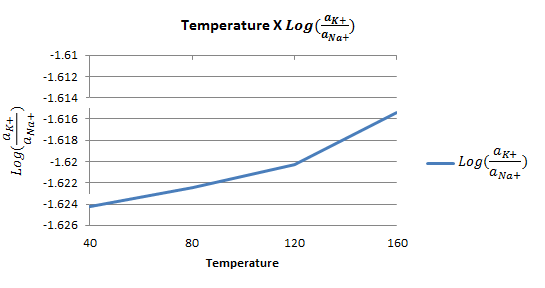
\includegraphics[width=100mm]{figures/tempXactratio.png}
\caption{Equilibrium diagram using the results from \emph{SHPECK}}
\label{fig:tempXactratio}
\end{figure}

% QUESTION:
% LEO: I wasn't sure if I should put the figure from aagaard's in order to really prove that our results are consistent.... 

\subsection{Computationally comparative} 
By modelling the same environment using three different software, we achieve a relevant comparison among the numerical methods and algorithms. 

The environment modelled is described in \cite{Morad:90} and the chemical composition of the water in \cite{Nordstrom:79}. The latter provides the chemical composition of the initial solution for the sea water. It can be verified the major components in table ~\ref{tab:nordstrom} - in $mM/L$. The temperature on this comparative study interpolate from $25^o$C to $160^o$C. In MINTEQA2, due restrictions to its thermodynamics equilibrium database, the maximal temperature available is $100^o$C.

\begin{table}
\caption{Chemical composition of the solution in the sea water at $25^o$C }
\label{tab:nordstrom}
\centering
\begin{tabular}{r|c|c|c|c|c|c|c|c|c}
\ce{Al^{3+}} & \ce{K^+} & \ce{Na^+} & \ce{Ca^{2+}} & \ce{Mg^{2+}} & \ce{Fe^{2+}} & \ce{SiO_2}&  
\ce{SO_4^{2-}} & \ce{Cl^-} & pH
    \\ \hline
7.59e-5 & 10.45 & 479.32 & 10.53 & 54.39 & 3.66e-5 & 0.073 & 28.893 & 559.5 & 8.22
\end{tabular}
\end{table}

The diagenetic processes modelled by the water-rock interactions are responsible for defining how of ions present the solution are going to behave. Figures ~\ref{fig:na+},~\ref{fig:cl-},~\ref{fig:mg+2},~\ref{fig:ca+2},~\ref{fig:k+} and ~\ref{fig:so4-2} present the most representative ions in the solution. It is possible to see that the behavior of \emph{SHPECK} accompany both \emph{PHREEQC} and \emph{MINTEQA2} in most of the cases, specially in temperatures under $100^o$C. We see a more distant behavior among \emph{SHPECK} and \emph{PHREEQC} in temperatures higher than $100^o$C but never completely opposites. This is explained due to temperatures where the equilibrium constant \emph{K} is not completely defined. This is a known issue from \emph{LLNL} thermodynamic dataset: sometimes equilibrium constants that are not measured are misterpreeted. \emph{SHPECK} uses the following approach: if there is one unknown equilibrium constant needed, it uses the closest known value. Unfortunately we can not describe exactly what other softwares do with this issue.

\begin{figure}[ht!]
\centering
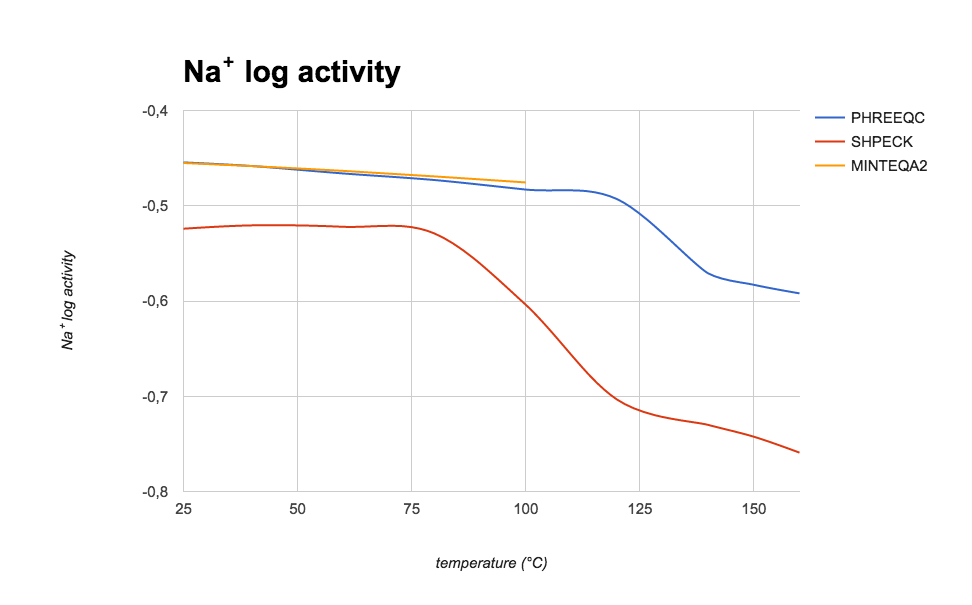
\includegraphics[width=140mm]{figures/na+.png}
\caption{\ce{Na^+} log activity comparative study}
\label{fig:na+}
\end{figure}

\begin{figure}[ht!]
\centering
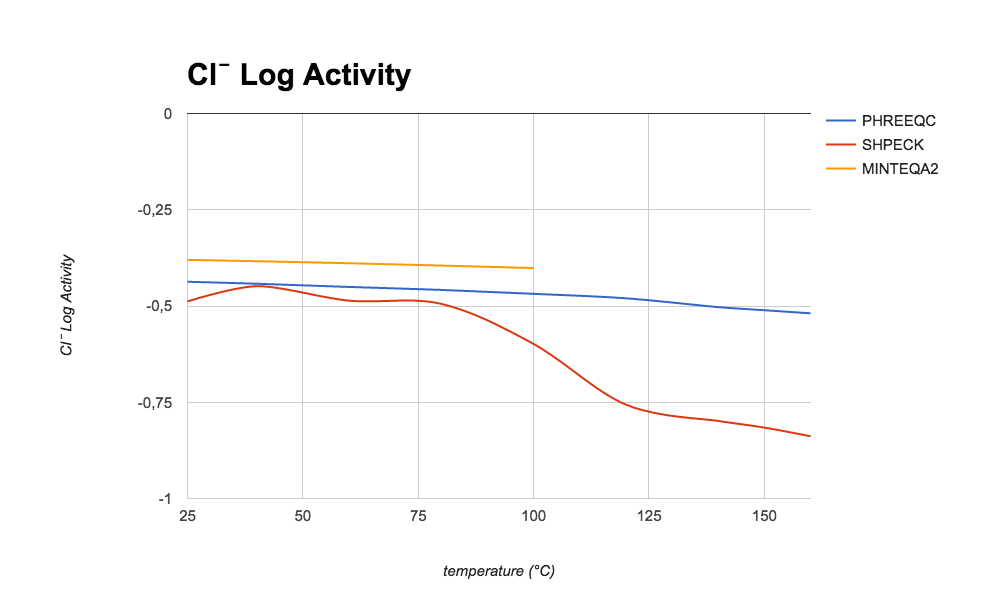
\includegraphics[width=140mm]{figures/cl-.png}
\caption{\ce{Cl^-} log activity comparative study}
\label{fig:cl-}
\end{figure}

\begin{figure}[ht!]
\centering
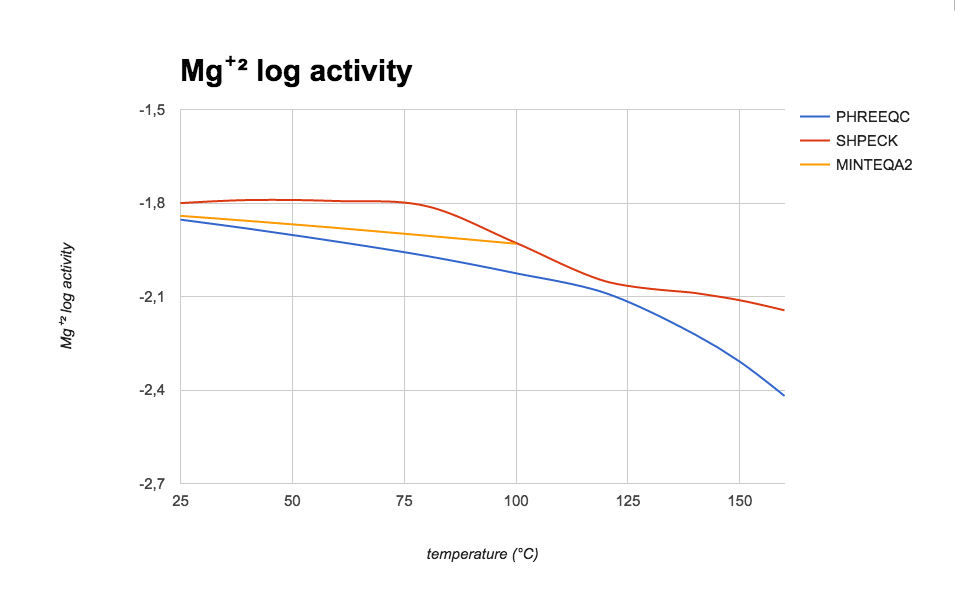
\includegraphics[width=140mm]{figures/mg+2.png}
\caption{\ce{Mg^{+2}} log activity comparative study}
\label{fig:mg+2}
\end{figure}

\begin{figure}[ht!]
\centering
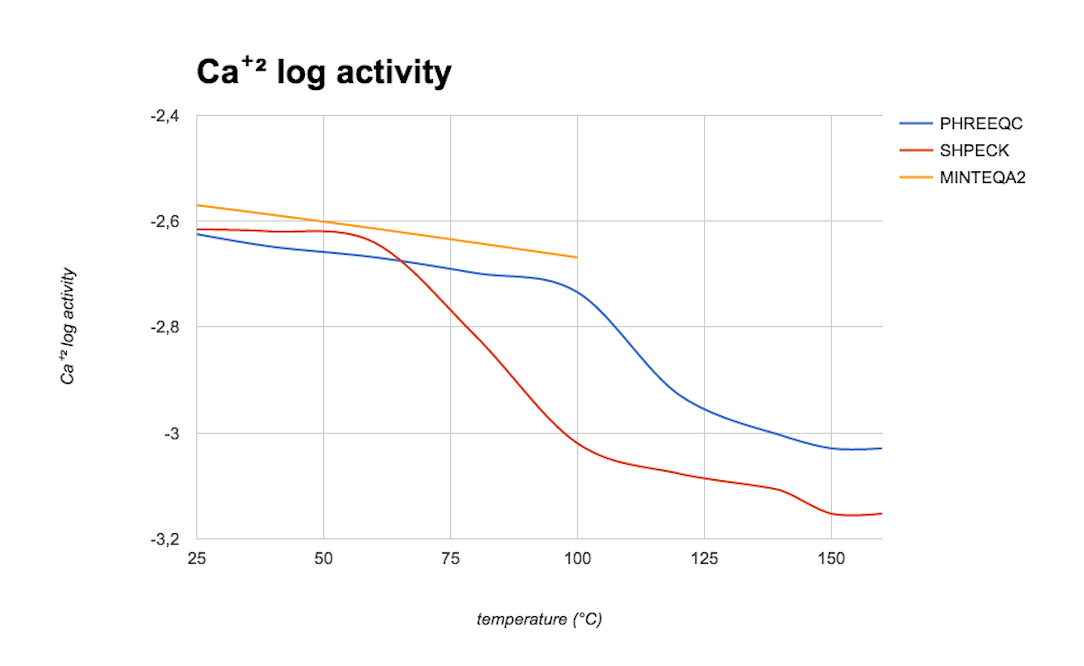
\includegraphics[width=140mm]{figures/ca+2.png}
\caption{\ce{Ca^{+2}} log activity comparative study}
\label{fig:ca+2}
\end{figure}

\begin{figure}[ht!]
\centering
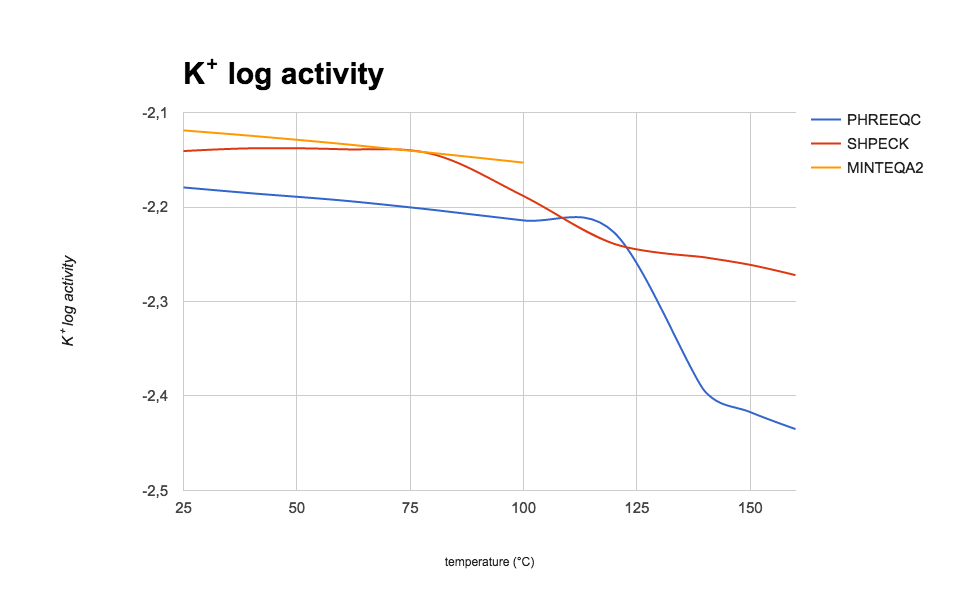
\includegraphics[width=140mm]{figures/k+.png}
\caption{\ce{K^+} log activity comparative study}
\label{fig:k+}
\end{figure}

\begin{figure}[ht!]
\centering
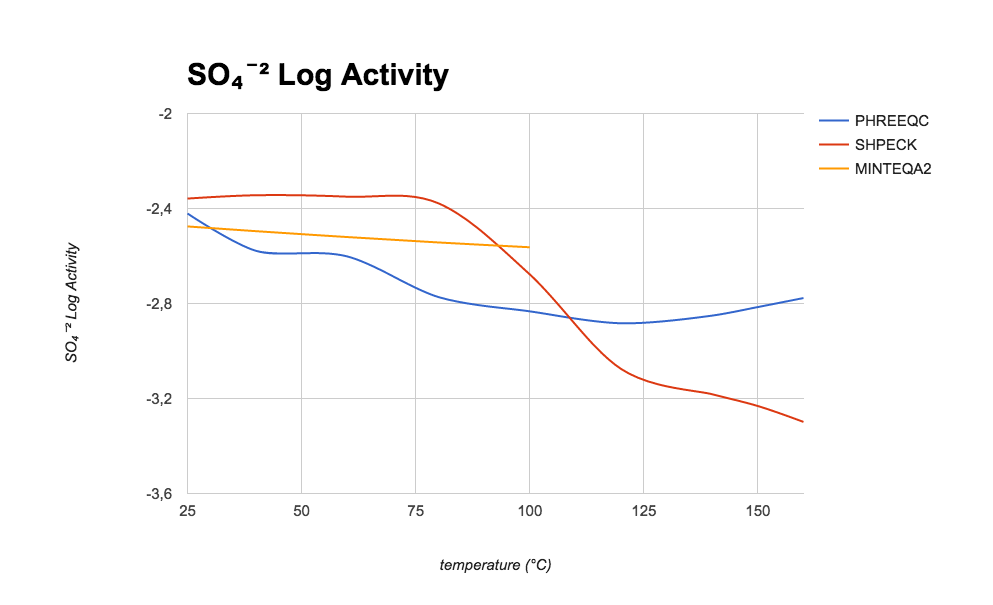
\includegraphics[width=140mm]{figures/so4-2.png}
\caption{\ce{SO_4^{-2}} log activity comparative study}
\label{fig:so4-2}
\end{figure}


\section{Database Evaluation}
The database is the source of every information inside a geochemical modelling software. The goal of this section is to make clear the difference and - more important - the benefits of \emph{SHPECK}'s relational database if compared to others. In geochemical modelling software the common approach is to use flat file databases; therefore, we're going to describe a time, space and expressiveness analysis between the \emph{LLNL} thermodynamic dataset and \emph{SHPECK}'s databse. 

Most of the information inside a geochemical database is related to each other (i.e. a mineral is described by a reaction, a reactio is composed by species, a specie is composed by elements). \emph{SQLite} databases are naturally a structure where the data can be related to each other, this affects drastically the performance and robustness of the application. On \emph{SQLite} databases, the data can be accessed using powerfull \emph{SQL} queries that reduce the complexity and increase the speed on information retrieval.

With flat file database, we have regular access to the information that it contains. In relation databases we use the \emph{SQL}. The studies in expressive power of query languages is one of the important fields in database studies - it studies the limitation and, on the other hand, the power of \emph{SQL}. Due to this works scope, we will not address basic knowledges in \emph{SQL} queries.

\subsection{Time analysis}
The response time is considered the sum of the processing time and the time waiting for the availabilit of the resource. It is fundamental for the performance of a geochemical modelling software to have fast access to the information since it is a bottleneck for the whole system. 
It is necessary to understand that until the software has received all the information requested from the database it will be doing nothing, completely stopped and waiting. This waste of CPU usage, if scaled to multiple simulations and long processing, is definitely something that can not be ignored. 
In order to analyze the response time with a geochemical analysis point of view, we discuss not only the access time but also what that information means.

When fetching any information from a thermodynamic dataset, it is important to take into consideration that no information actually matters if considered alone; there will always be supporting information to get also - which menas more database searches and consuming time. For example, when fetching a reaction (as expressed in equation ~\ref{reaction}), the basic informations are the compounds that take part on this reaction and the related stoichiometric values. Behind this action, the database must also provide informations about the compounds itself (i.e. charge, ion size, mole weigth, elements in that specie, formula, mole volume, thermodynamic equilibrium constant coefficients, etc). 

Figure ~\ref{fig:timeXaccess} indicate the time elapsed (in seconds) that it costs to retrieve all the information related to a chemical reaction from the database. In this example, we simulated from 20 to 580 reactions randomly in the database.

\begin{figure}[ht!]
\centering
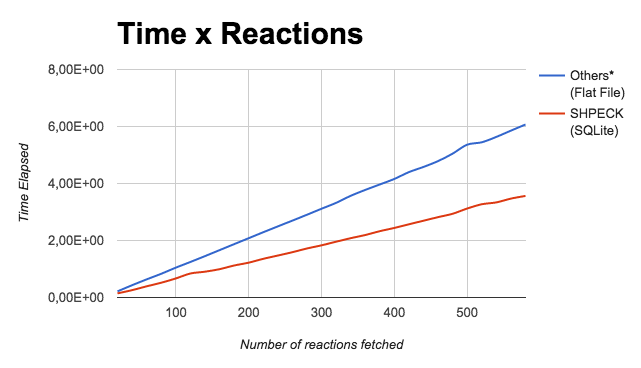
\includegraphics[width=140mm]{figures/timeXreactionAccess.png}
\caption{Time elapsed in seconds X Reactions Accessed}
\label{fig:timeXaccess}
\end{figure}


\newpage
\section{Summary}
\begin{itemize}
    \item Diagenesis: This term refers to the physical-chemical reactions responsible for the compaction and precipitation of minerals  during the generation, migration and storage of oil. Understand how these reactions actually occur is fundamental to be able to predict porosity, solubility and permeability of reservoirs and using geochemical modelling softwares is one effective and accessible way to learn about this complex environment.
    \item Study case: We reproduce the diagenetic reactions observed in Snorre Field reservoir sandstones, Norwegian's North Sea. The environment modelled is described in \cite{Morad:90} and the chemical composition of the water in \cite{Nordstrom:79}.
    \item Comparative study: We perform a comparative study with \emph{SHPECK} side-by-side with others available geochemical speciation softwares. The results prove that \emph{SHPECK} reach good results with high accuracy. The discrepancies are minimal and are expected since each software has its own mathematical and computational treatment to the set of equations, parameters, activity coefficient calculation methods and thermodynamic dataset interpretation. 
    \item Database evaluation: The lack of a relational database in the geochemical modelling softwares makes clear that none of the existing options were really developed with a computer science emphasis. \emph{SHPECK} uses a \emph{SQLite} database specially developed to support a geochemical speciation modelling software. This software design option enables our software to achieve a higher performance, handle complex queries and fetch relevant information easier. A comparative graph highlights the advantages in time elapsed by the number of reactions requested as an exercise to detect this.
\end{itemize}